\chapter{Ingénierie des exigences}
\section{Approche Top-Down}
\label{sec:top-down}

Pour notre approche Top-Down, nous sommes revenus à la demande initiale du projet : remplacer la souris d'un ordinateur par le mouvement oculaire de l'utilisateur. La fonction principale du système est donc apparue clairement : permettre à l'utilisateur d'interagir avec une interface via ses yeux. 

\begin{figure}[h]
  \centering
  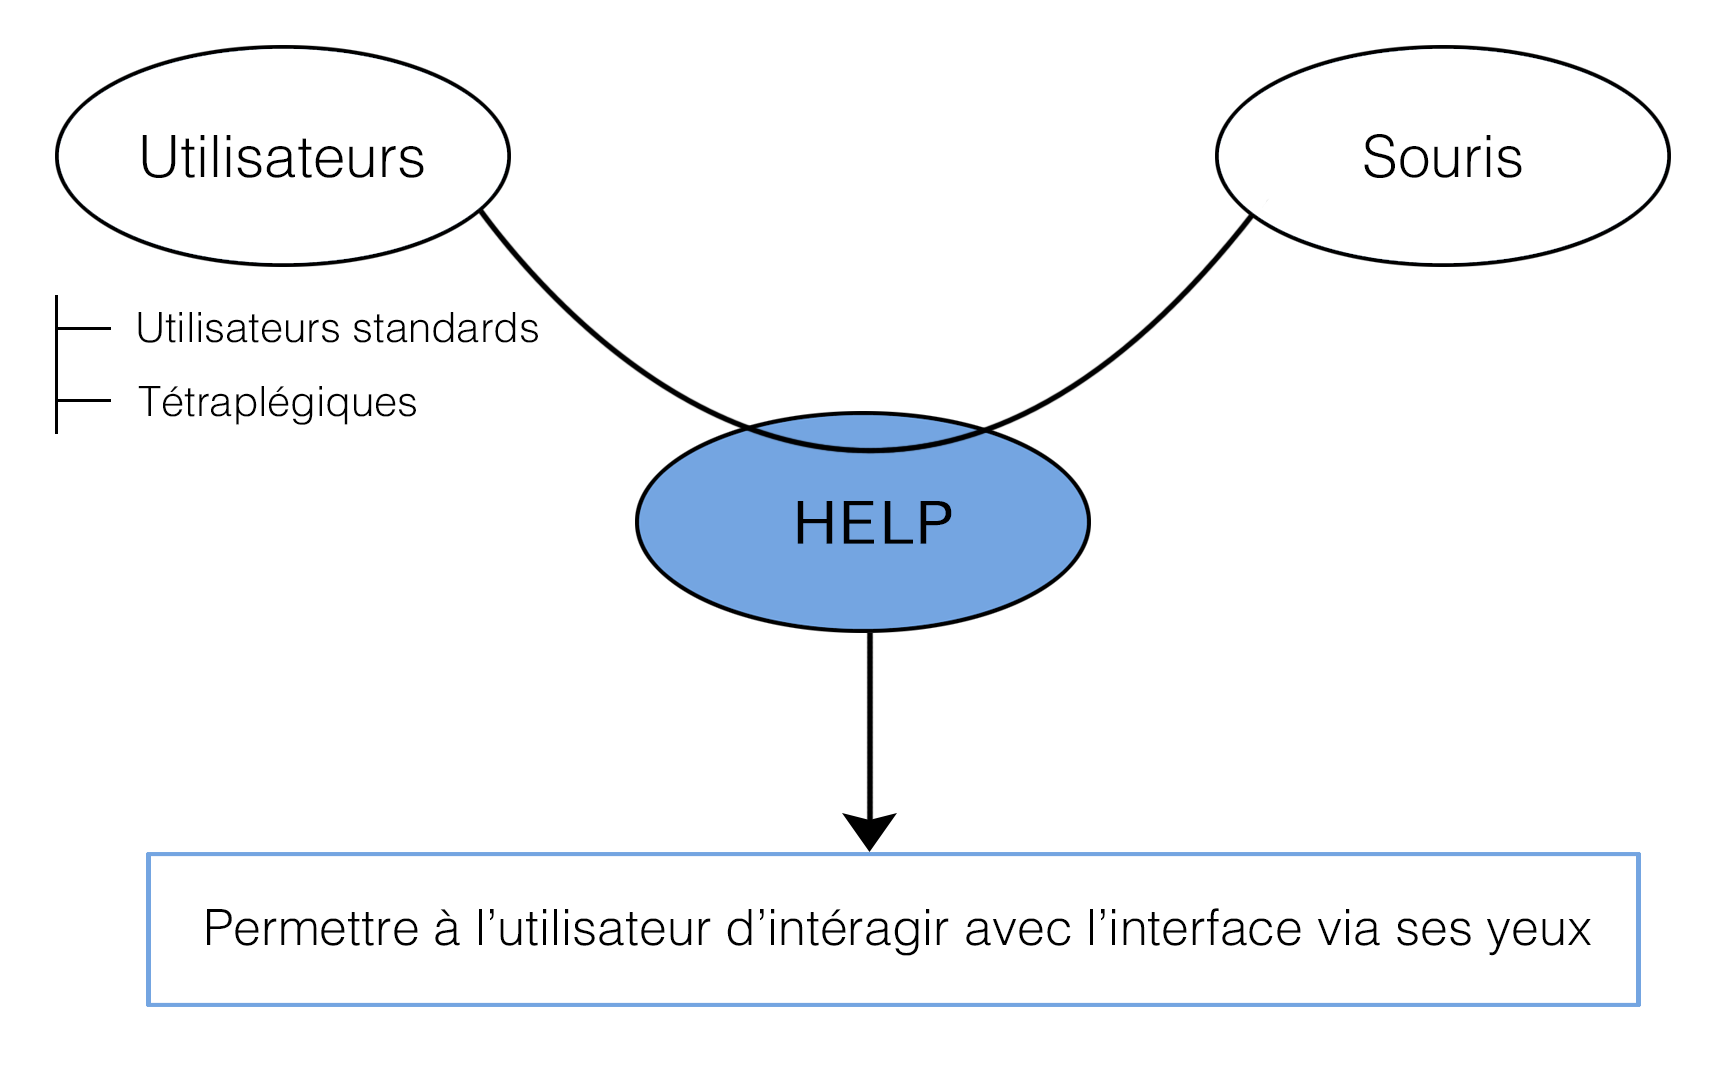
\includegraphics[scale=1]{BeteACornes}
  \caption{Bête à cornes}
  \label{fig:bac}
\end{figure}

\begin{figure}[H]
  \centering
  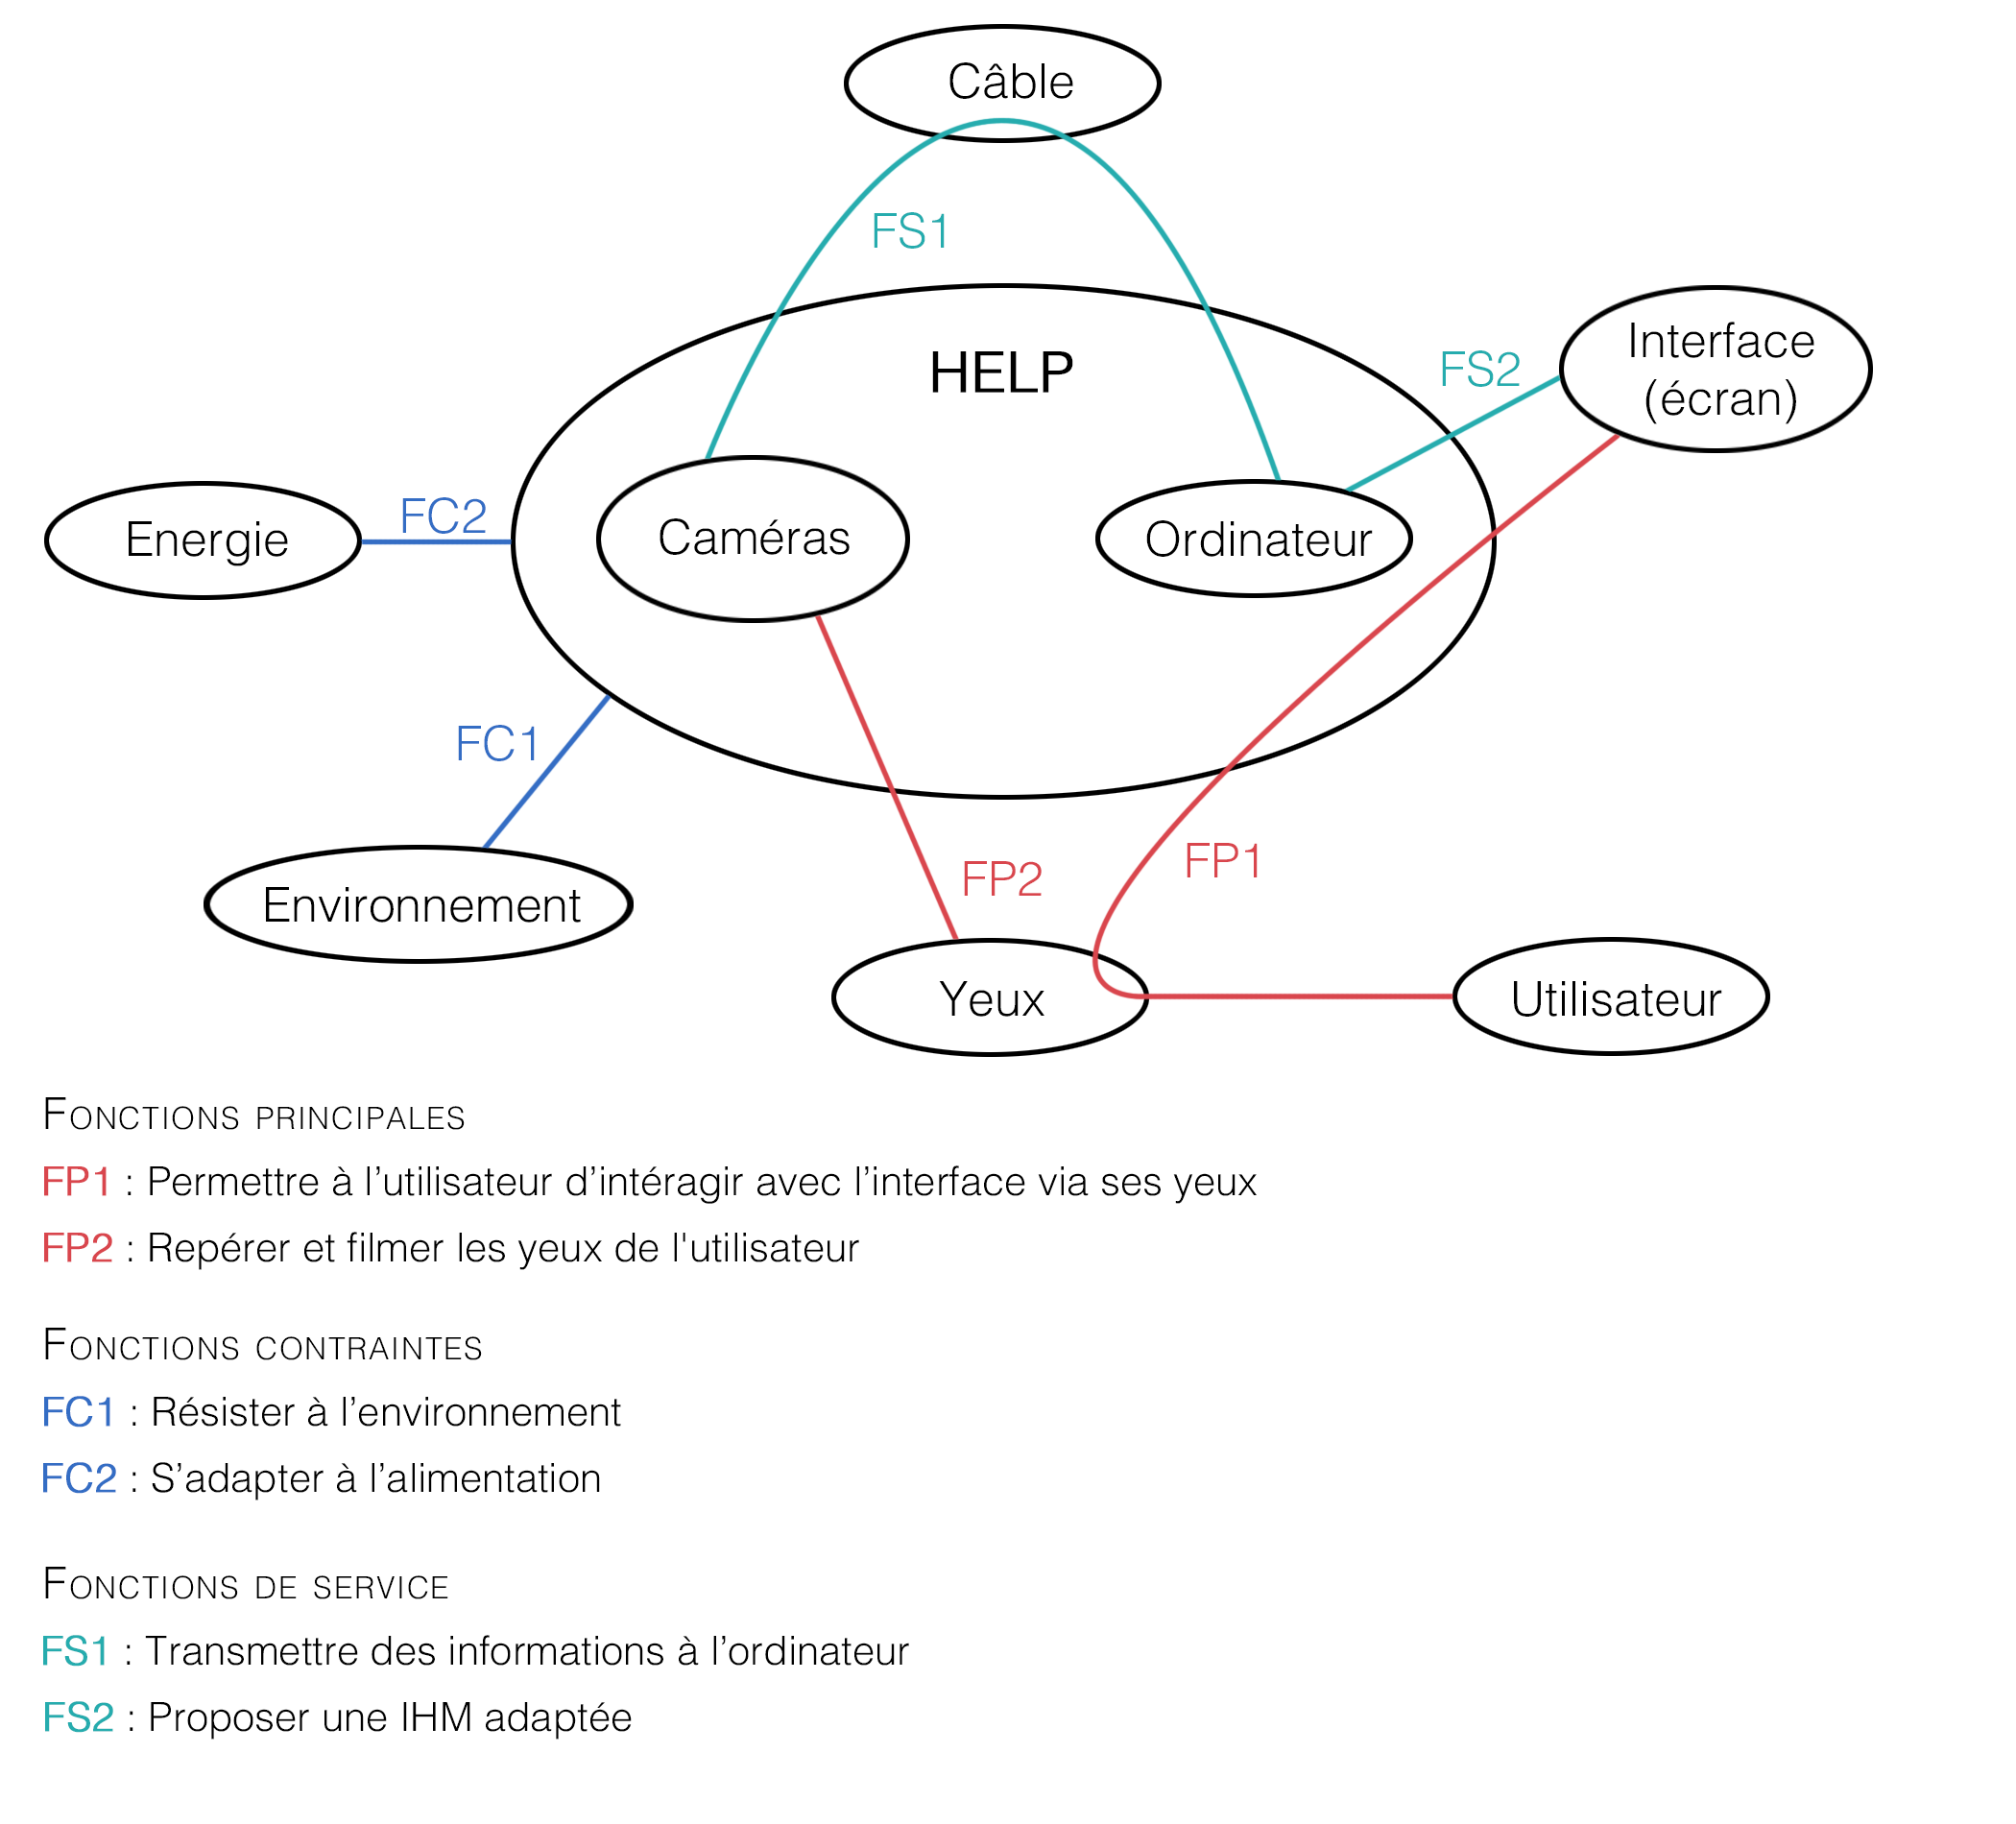
\includegraphics[scale=0.9]{PieuvreV2}
  \caption{Diagramme pieuvre}
  \label{fig:pieuvre}
\end{figure}

\section{Approche Bottom-Up}
\definecolor{sable}{RGB}{238,236,225}
Nous avons défini les différentes exigences auxquelles le système devra répondre, indépendamment de nos choix de réalisation technique. Nous les avons alors rassemblées par groupement logique, ce qui nous permettra de définir nos fonctions principales. Les lignes en {\color{sable}{\rule{0.5cm}{0.25cm}}} sont uniquement valables pour la méthode embarquant un système sur l'utilisateur. Elles sont donc à ignorer dans un premier temps puisque nous avons choisi une approche différente. 

\begin{figure}[H]
  \centering
  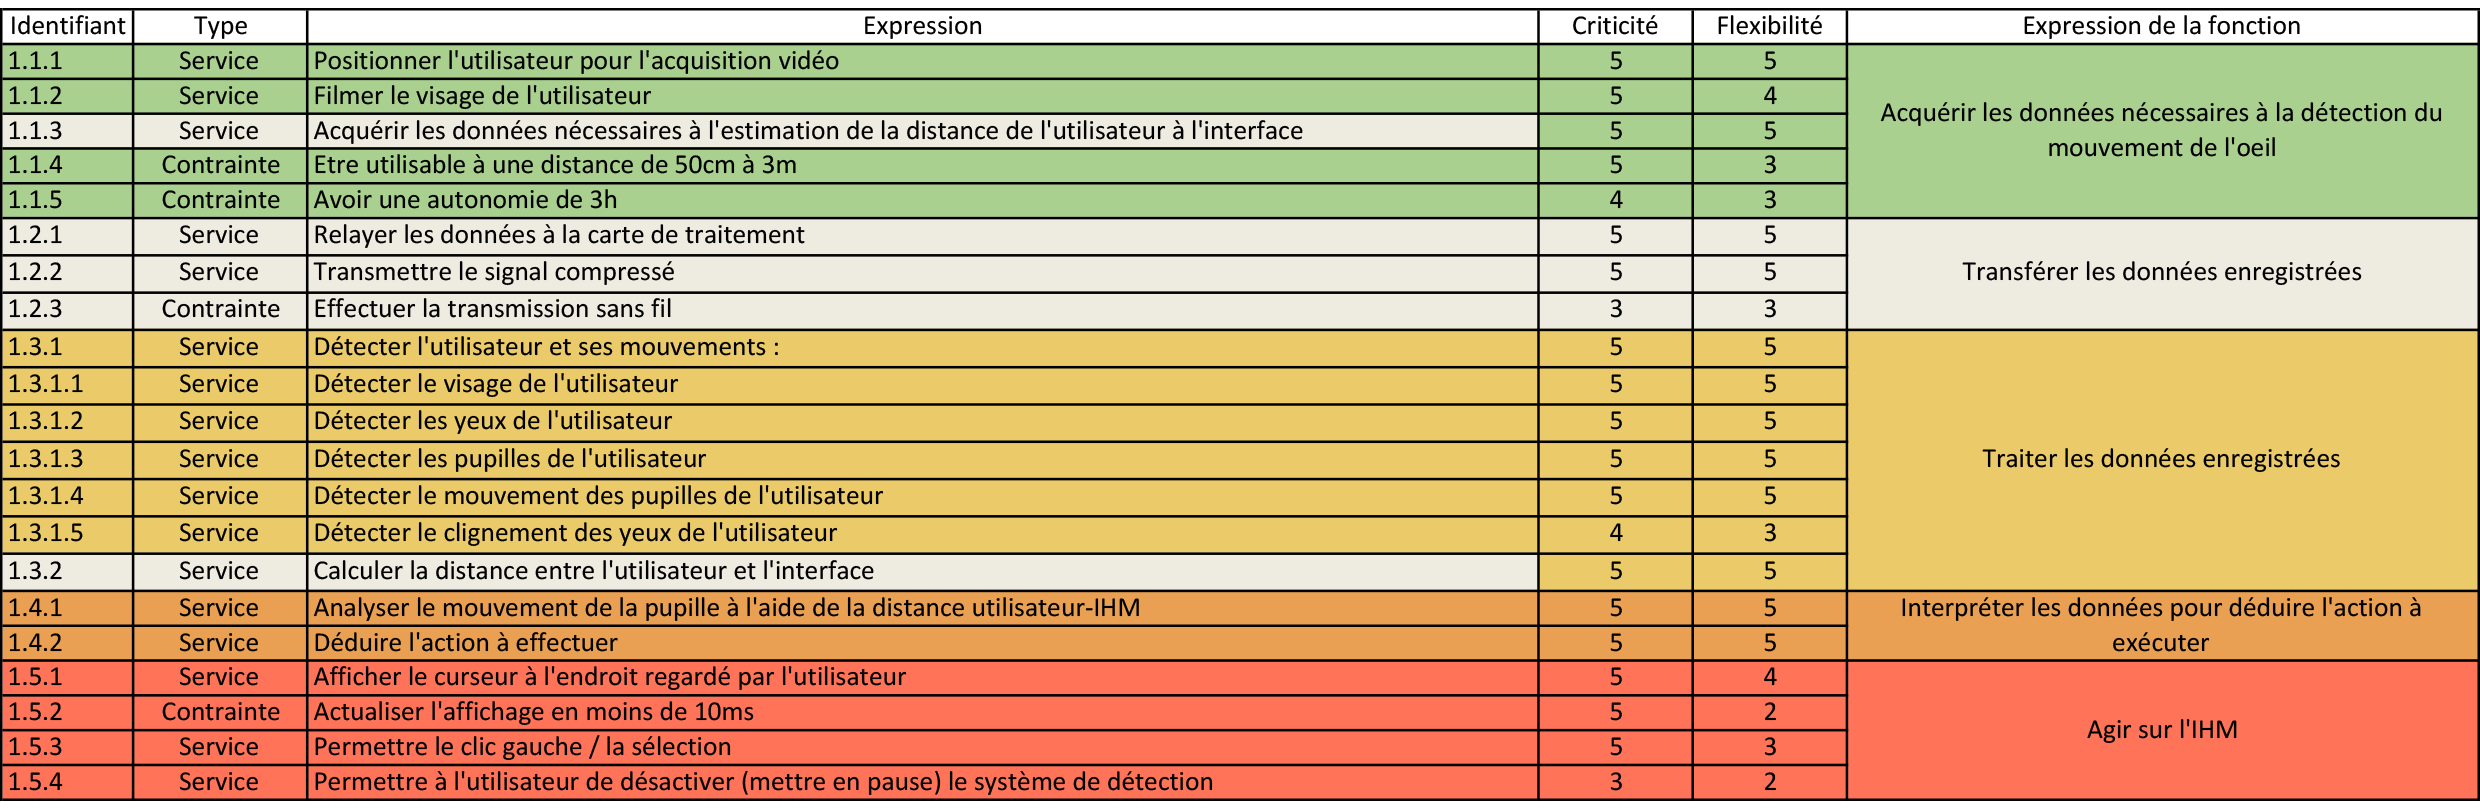
\includegraphics[width=\textwidth]{CahierdesExigencesV2}
  \caption{Cahier des exigences}
  \label{fig:exigences}
\end{figure}

\section{Fonctions principales du système}

Dans le cadre de ce projet, nous cherchons donc à remplacer la souris d'un ordinateur par un système qui suit le mouvement des yeux de l'utilisateur. Pour ce faire, nous avons mis en évidence des groupements logiques d'exigence. Tout d'abord, le système doit acquérir les données nécessaires à la détection du mouvement de l'œil. Ces données devront alors être traitées par l'ordinateur. Ce dernier doit alors interpréter ces données pour en déduire l'action à exécuter. De ces nouvelles informations, l'ordinateur doit pouvoir effectuer l'action que l'utilisateur veut effectuer sur l'IHM, la mettre en place, et montrer que ces modifications ont été exécutées. 

\begin{itemize}[label=\textbullet,font=\color{black}]
\item FP1 : Acquérir les données nécessaire à la détection du mouvement de l'œil 
\item\colorbox{sable}{FP2 : Transférer les données enregistrées}
\item FP3 : Traiter les données enregistrées 
\item FP4 : Interpréter les données pour déduire l'action à exécuter 
\item FP5 : Agir sur l'IHM 
\end{itemize}

\chapter{Spécification fonctionnelle  3 axes}

\section{Raffinement FAST}

\begin{figure}[h]
  \centering
  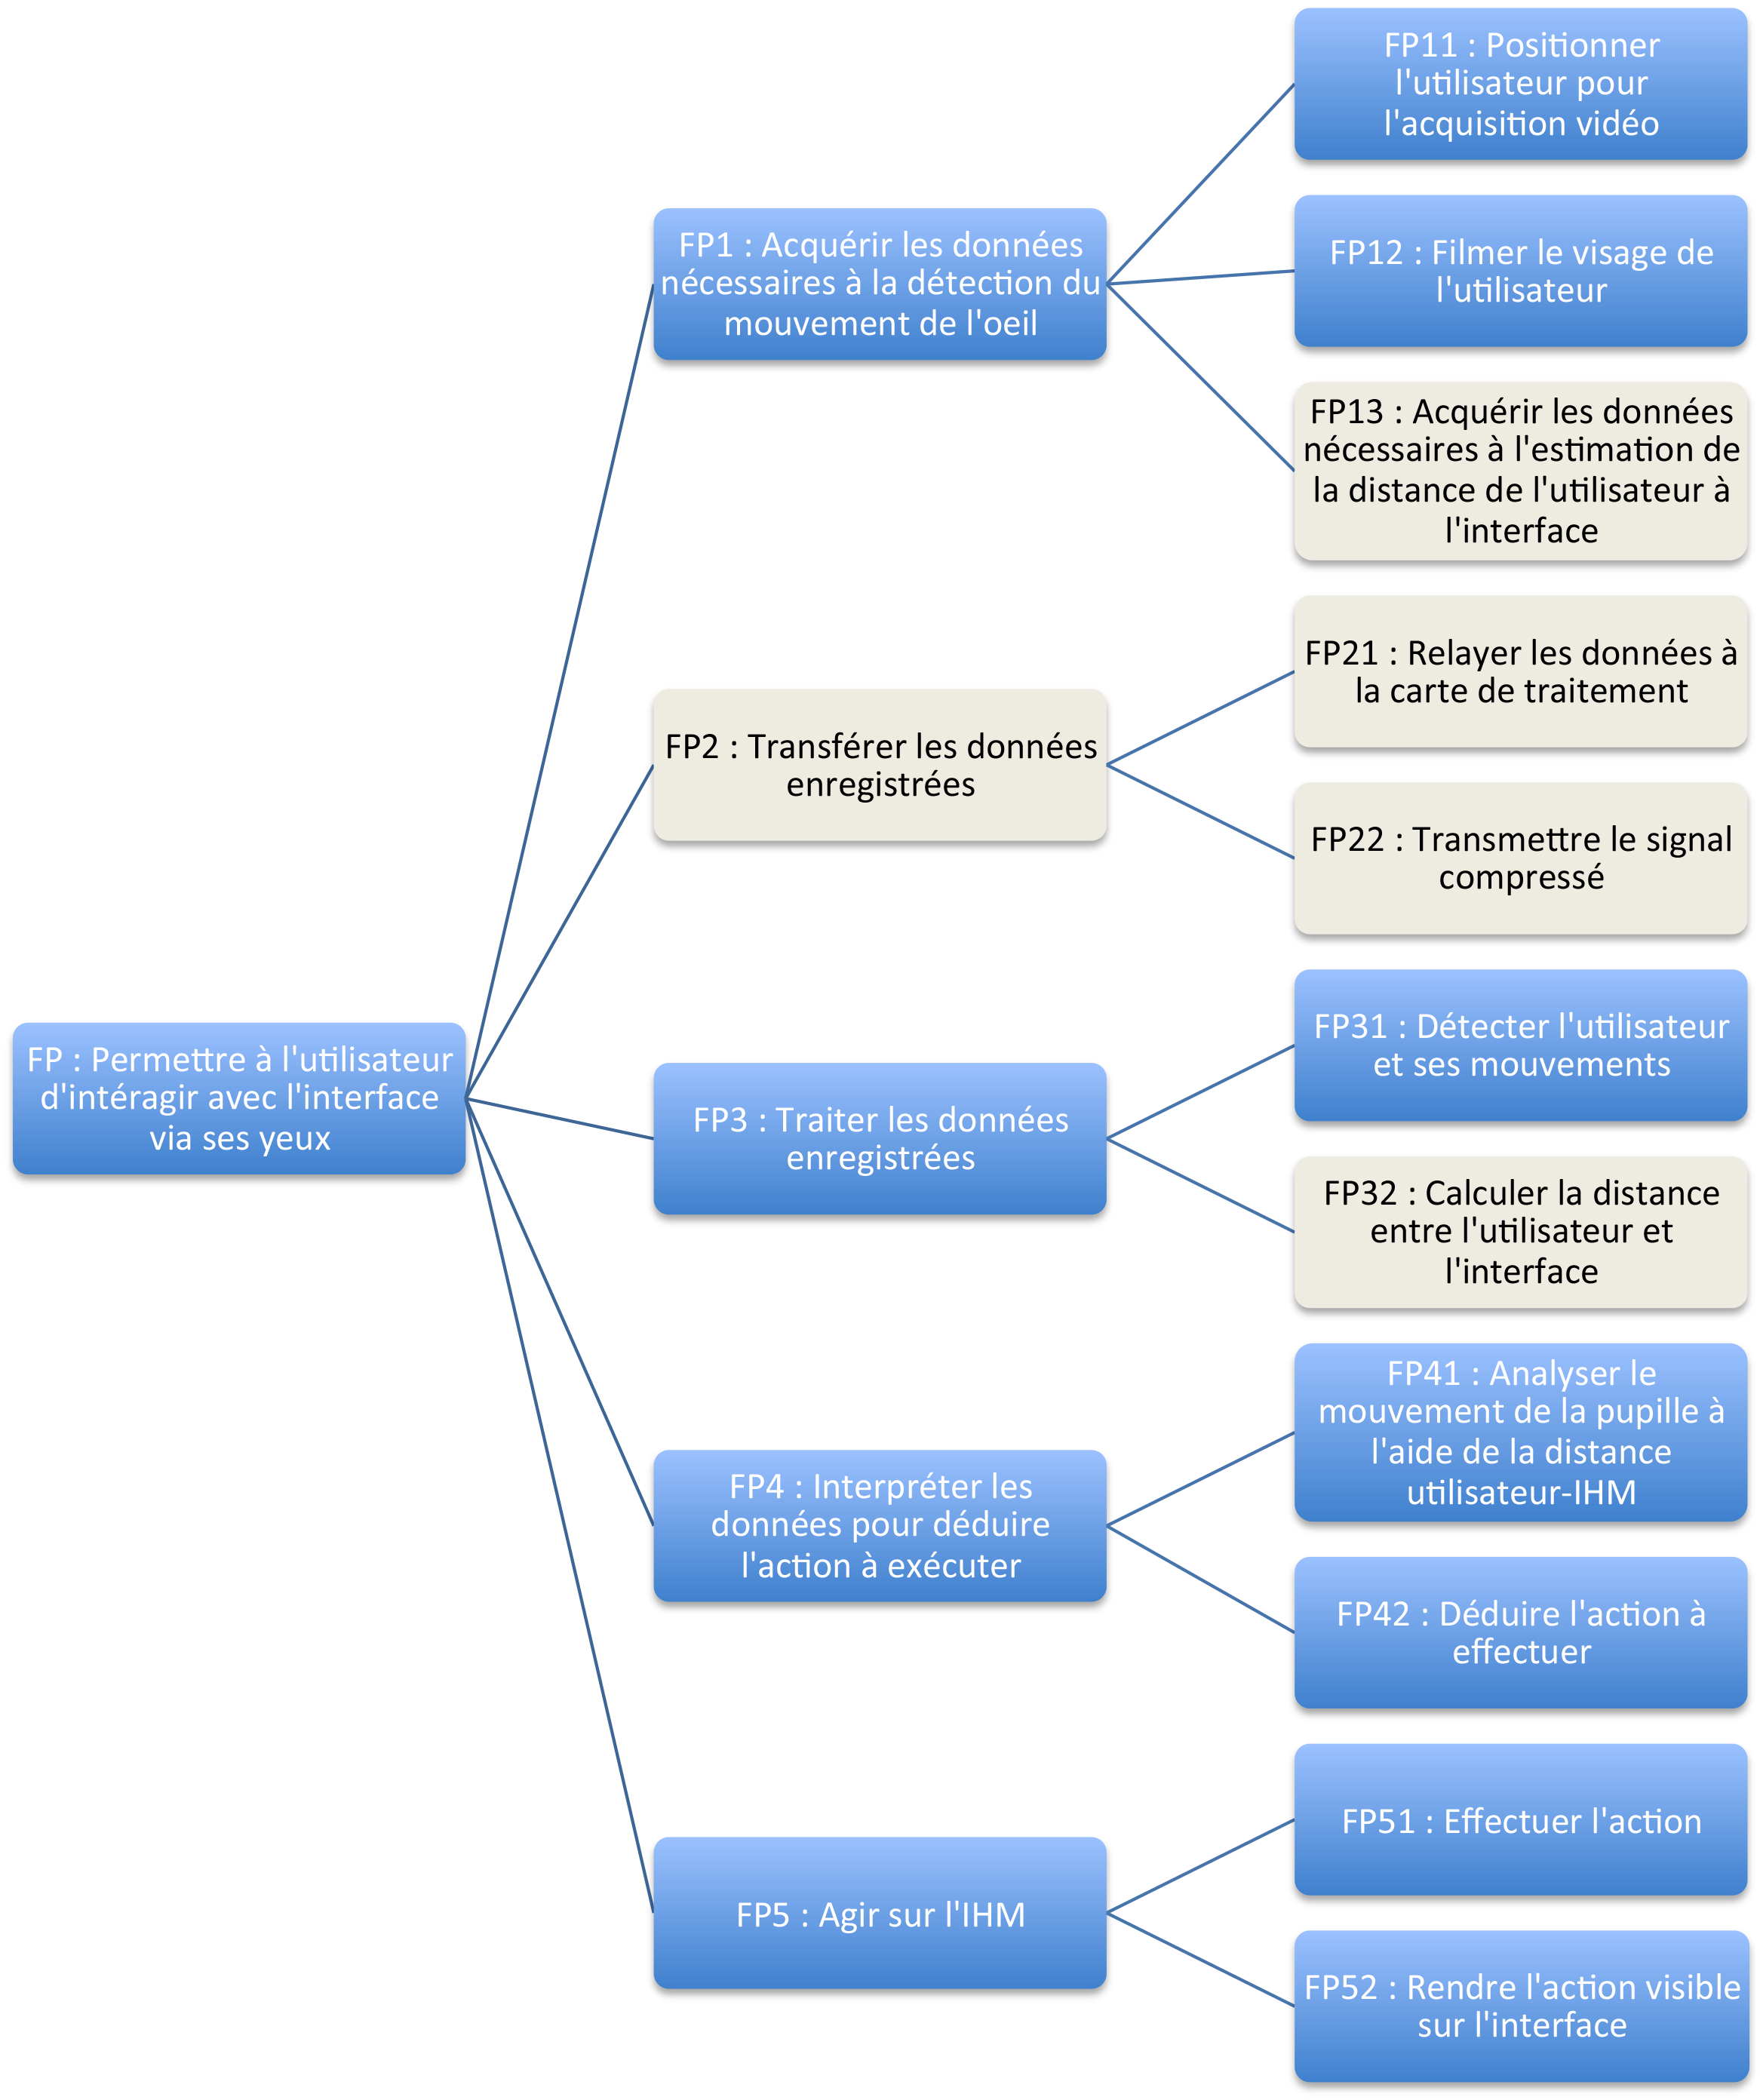
\includegraphics[scale=0.75]{FASTV2}
  \caption{FAST raffiné}
  \label{fig:FAST}
\end{figure}

Le cahier des exigences précédant nous a permis de définir les fonctions principales du système. Nous avons alors cherché à les raffiner par la méthode FAST (cf. figure \ref{fig:FAST}) pour obtenir des fonctions plus précises auxquelles nous pourront apporter des solutions techniques propres à chacune. Nous pouvons ainsi entrevoir l'architecture fonctionnelle.

\section{Spécification des données}
\begin{figure}[h]
  \centering
  \includegraphics[scale=0.6]{fluxDonnees}
  \caption{Flux de données}
  \label{fig:fluxDonnees}
\end{figure}

%\section{Spécification des comportements}

\chapter{Architecture fonctionnelle}

Tout le travail réalisé au préalable sur la spécification fonctionnelle 3 axes permet finalement de proposer une architecture fonctionnelle pour notre système (cf. figure \ref{fig:archiFonctionnelle}).
 
\begin{figure}[h]
  \centering
  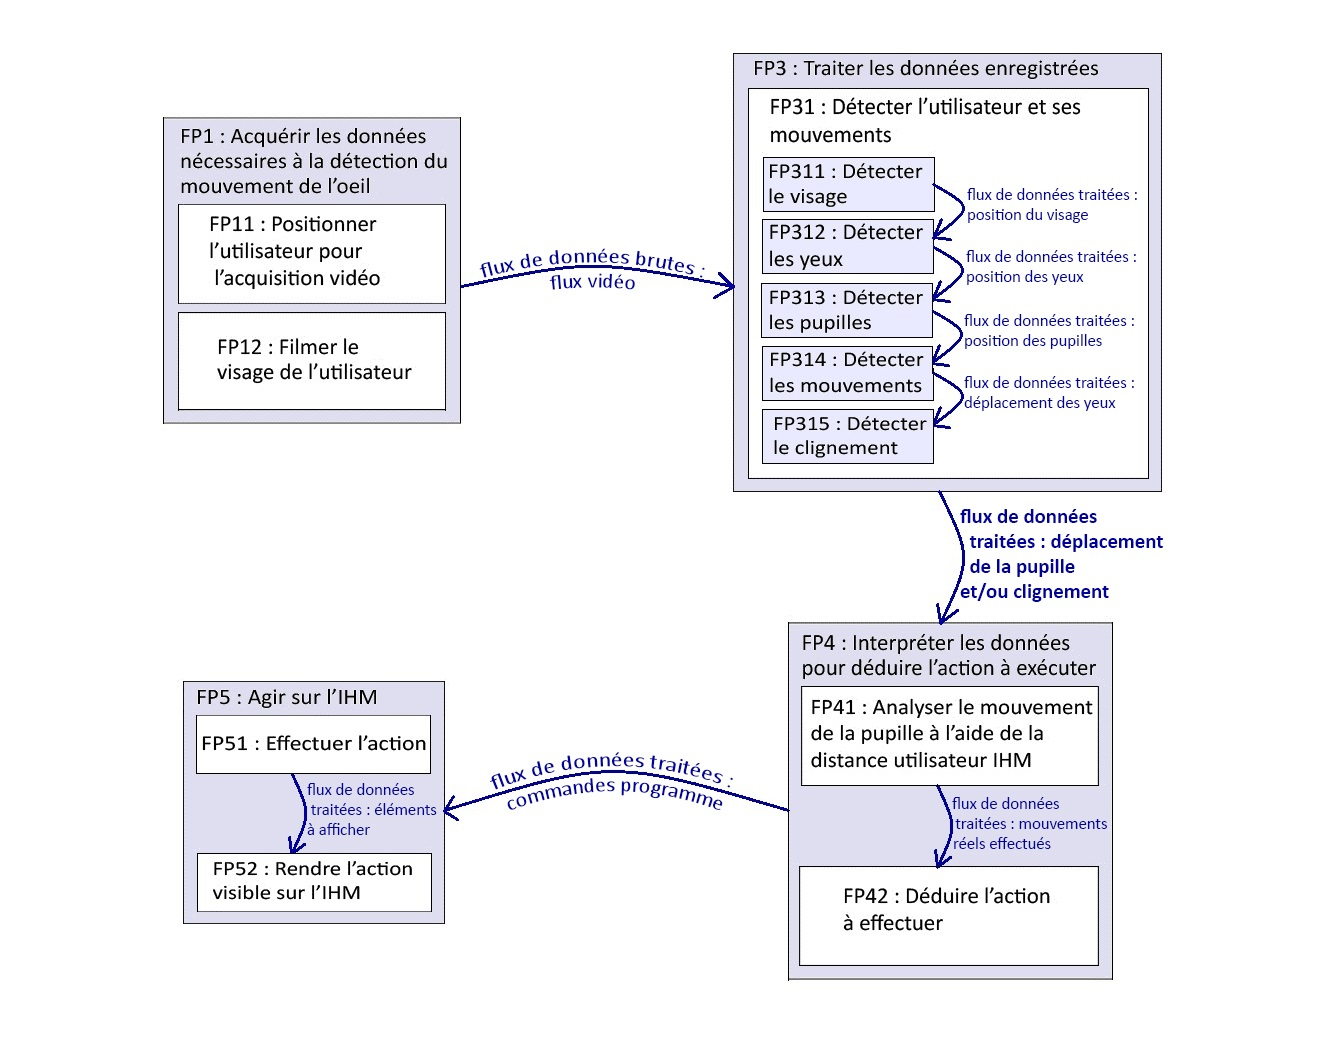
\includegraphics[scale=1.2]{ArchitectureFonctionnelletxt}
  \caption{Architecture Fonctionnelle}
  \label{fig:archiFonctionnelle}
\end{figure}

